% Chapter Template

\chapter{Reti Neurali Convoluzionali} % Main chapter title
\label{Capitolo3}
\def \teoria {Figures/teoria}
\def \path	 {Figures/C3}
%--------------------------------------------------------------------%	SECTION 1
%--------------------------------------------------------------------
%% da completare
In questo capitolo si introduce una panoramica generale sulle reti neurali convoluzionali. Essendo un argomento vasto, una trattazione teorica approfondita sarebbe materia di una tesi di laurea, ragion per cui gli argomenti sono introdotti con lo scopo di avere un'infarinatura per comprendere le applicazioni sviluppate nei capitoli successivi. 
\section{Breve introduzione}
La reti neurali convoluzionali, alle quali ci riferiremo con l'abbrevazione \emph{CNN} - dall'inglese \emph{Convolutional Neural Network}, sono un'evoluzione delle normali reti artificiali profonde caratterizzate da una particolare architettura estremamente vantaggiosa per compiti visivi (e non), che le ha rese negli anni molto efficaci e popolari. Sono state ispirate dalle ricerche biologiche di Hubel e Wiesel i quali, studiando il cervello dei gatti, avevano scoperto che la loro corteccia visiva conteneva una complessa struttura di cellule. Quest'ultime erano sensibili a piccole parti locali del campo visivo, detti campi recettivi \emph{(receptive fields)}. Agivano quindi da filtri locali perfetti per comprendere la correlazione locale degli oggetti in un'immagine. Essendo questi sistemi i più efficienti in natura per la comprensione delle immagini, i ricercatori hanno tentato di simularli. 

%--------------------------------------------------------------------
%	SECTION 2
%--------------------------------------------------------------------

\section{Architettura}
Le CNN sono reti neurali profonde costituite da diversi strati che fungono da estrattori delle features ed una rete completamente connessa alla fine, che funge da classificatore, come raffigurato in figura \ref{fig:cnn1}. \\
\begin{figure}[h!]
 \centering
 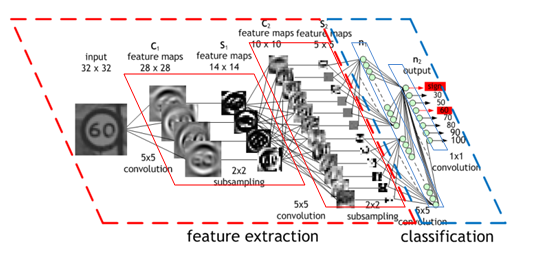
\includegraphics[width=1.0\textwidth]{\path/CNN-expl.png} 
 \caption{Architettura di una CNN che classifica segnali stradali: si evidenzia la divisione tra gli strati che fungono da feature extractor ed il classificatore finale}
 \label{fig:cnn1}
\end{figure}
Questi strati in cui si estraggono le caratteristiche delle immagini sono detti strati di convoluzione, e sono generalmente seguiti da una funzione non lineare e un passo di \emph{pooling}. Vi possono poi essere degli strati di elaborazione dell'immagine, come quello di normalizzazione del contrasto, si veda \fig{ref:cnn2}.
%%% ricollocare la figura %%% 
\begin{figure}[h!]
 \centering
 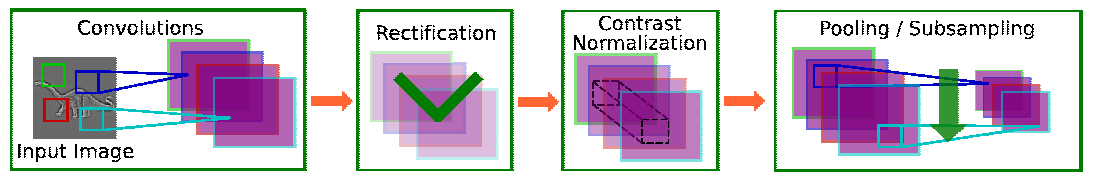
\includegraphics[width=1.0\textwidth]{\path/CNN-features.png} 
 \caption{I diversi strati tipici di una CNN}
 \label{fig:cnn2}
\end{figure}
Convoluzione e pooling hanno come scopo quello di estrarre le caratteristiche, mentre l’unità non lineare serve a rafforzare le caratteristiche più forti e indebolire quelle meno importanti, ovvero quelle che hanno stimolato meno i neuroni (si dice che fa da “squashing”). \\
Sempre dalla figura \ref{fig:cnn1}, possiamo inoltre notare che, per ogni immagine in input, corrispondono nei vari strati, diversi gruppi di immagini, che vengono chiamate \emph{feature maps}. Le feature maps sono il risultato dell'operazione di convoluzione svolta tramite un banco di filtri, chiamati anche kernel, che altro non sono che delle matrici con dei valori utili a ricercare determinate caratteristiche nelle immagini.\\
Infine, terminati i convolutional layers, le feature maps vengono “srotolate” in vettori e affidate ad una rete neurale "classica" che esegue la classificazione finale. 

Il numero di strati di convoluzione è arbitrario. Inizialmente, quando le CNN divennero famose grazie a Y.LeCun, che addestrò una CNN chiamata \emph{"LeNet5"} al riconoscimento dei numeri \parencite{lenet}, questo numero era compreso tra 2-5. Nel 2012, Alex Krizhevsky et al \parencite{imagenet2012} addestrarono una rete costituita da 5 strati di convoluzione, 60 milioni di parametri e 650 mila neuroni. Ottennero la migliore percentuale d'errore al mondo sul dataset ImageNet ILSVRC-2010, contenente 1,2 milioni di immagini divise in 1000 categorie. \\
Da allora le cose si sono evolute con una velocità disaramente, e l'ImageNet challenge del 2015, è stata vinta da una rete con 152 strati \parencite{resnet}. Nel capitolo \ref{Capitolo5} si farà un confronto tra quest'ultima rete, soprannominata \emph{"ResNet"} e la capostipite LeNet5 su un task di classificazione.   
\subsection{Strato di Convoluzione}
Per comprendere appieno quello che avviene in una CNN, occorre introdurre il concetto di convoluzione fra matrici, e capire come questo sia importante per applicare dei filtri ad un'immagine digitale.
\\
Un’immagine digitale può essere considerata come una matrice A di dimensione MxN valori reali o discreti. Ogni valore della matrice prende il nome di pixel e i suoi indici sono anche chiamati coordinate: ogni pixel $A(m,n)$ rappresenta l’intensità nella posizione indicata dagli indici. \\ 
Si definisce “filtro” o “kernel” una trasformazione applicata ad un’immagine. Come detto prima, questi filtri sono a loro volta della matrici; la trasformazione quindi si effettua appunto tramite un'operazione di convoluzione tra l'immagine in ingresso ed il filtro.
La convoluzione, discreta nel caso di immagini digitali, si può definire come: 
%% INSERIRE EQUZIONEI %%% 
$$
y[m,n] = x[m,n] \circledast h[m,n] = \sum^{m}\sum^{n}x[i,j]\times h[m-i,n-j]
$$
Ogni pixel di $y[m,n]$ è così il risultato di una somma pesata tramite $h[m,n]$ della sottoregione che ha centro nel pixel indicato dalle coordinate m,n. Un esempio di convoluzione è rappresentato in figura \ref{fig:convolution}. 
\begin{figure}[h!]
 \centering
 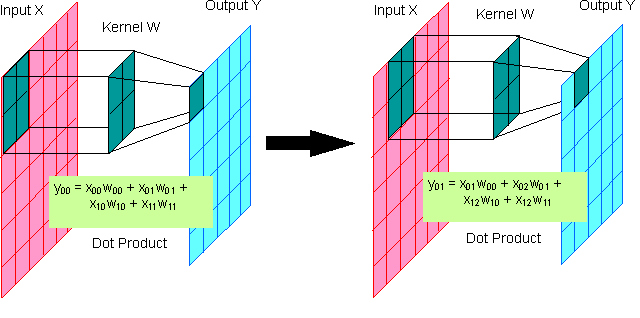
\includegraphics[width=0.7\textwidth]{\path/convolution.png} 
 \caption{Convoluzione con un kernel: primi due step}
 \label{fig:convolution}
\end{figure}
\\
Nei convolutional layers viene quindi fatta un'operazione di convoluzione tra l'immagine/i in ingresso
e un numero arbitrario K di filtri. Questi filtri hanno valori tali da ottenere in uscita un riconoscimento di determinate caratteristiche. \\
I valori dei filtri sono all'inizio scelti casualmente, e vengono poi migliorati ad ogni iterazione mediante l'algoritmo di backpropagation, visto nel Capitolo \ref{Capitolo2}. Così facendo la rete addestra i suoi filtri ad estrarre le features più importanti degli esempi del training set; cambiando training set i valori dei
filtri saranno diversi.
Ad esempio, i valori dei filtri di una rete allenata con immagini di pali verticali saranno diversi da quella allenata con immagini di palloni da calcio; nel primo caso i valori saranno calibrati per riconoscere lunghi orientamenti verticali, mentre
nel secondo per riconoscere i confini sferici. 

Nelle reti convoluzionali quindi, l'algoritmo di Backpropagation migliora i valori dei filtri della rete, è lì quindi che si accumula l'apprendimento. I neuroni, in queste reti, devono intendersi come i singoli filtri.\\
\\
Vi sono diversi \emph{hyperparameters} da settare manualmente negli strati di convoluzione: 
\begin{enumerate}
\item la misura del filtro $F$: chiamato anche \emph{receptive field}. Ogni filtro cerca una determinata caratteristica in un'area locale dell'immagine, la sua misura quindi è il campo recettivo del singolo neurone. Tipicamente sono 3x3, 5x5 o 7x7.

\item il numero $K$ di filtri: per ogni strato, questo valore definisce la profondità dell'output dell'operazione di convoluzione. Infatti, mettendo una sopra l'altra le feature maps, si ottiene un cubo in cui ogni "fetta" è il risultato dell'operazione tra l'immagine in ingresso ed il corrispettivo filtro. La profondità di questo cubo dipende appunto dal numero dei filtri. 

\item lo \emph{"Stride"} S: definisce di quanti pixel si muove il filtro della convoluzione ad ogni passo. Se lo stride è settato a 2, il filtro salterà 2 pixel alla volta, producendo quindi un output più piccolo. 

\item il \emph{"padding"} P: definisce la misura con la quale si vuole aggiungere degli "0" all'input per preservare la dimensione in output. In generale, quando lo stride S=1, un valore di  $P = (F - 1)/2$ garantisce che l'output avrà le stesse dimensioni dell'input. 
\end{enumerate}
\\
%% pezzo sulla dimensione in output %% 
Quando si elaborano delle immagini con le CNN si hanno generalmente in ingresso degli input tridimensionali, caratterizzati dall'altezza $H_1$, l'ampiezza $W_1$ e il numero di canali di colore $D_1$. Conoscendo i parametri sopra specificati si può calcolare la dimensione dell'output di un layer di convoluzione: 
\begin{align*}
H_2 = (H_1 - F + 2P)/S + 1\\
W_2 = (H_1 - F + 2P)/S + 1\\
D_2 = K
\end{align*}
%% 
A questo proposito si osservi un esempio di "volume di neuroni" del primo strato di convoluzione in figura \ref{fig:depth}. Ogni neurone è collegato spazialmente solo ad 1 regione locale dell'input ma per tutta la profondità (i.e. i 3 canali del colore). Si noti che ci sono 5 neuroni lungo la profondità e tutti guardano alla stessa regione dell'input.
\begin{figure}[h!]
 \centering
 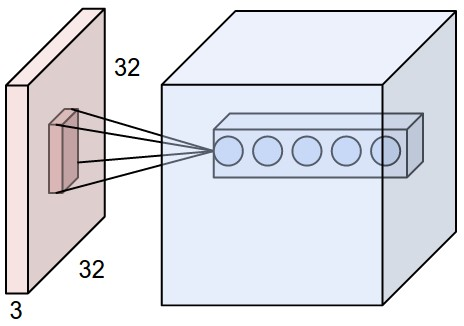
\includegraphics[width=0.4\textwidth]{\path/depthcol.jpeg} 
 \caption{Ogni neurone è connesso a solo 1 regione locale dell'input ma a tutta la profondità (i.e. canali colori). La depth dell'output è data dal numero K di filtri, in questo caso 5}
 \label{fig:depth}
\end{figure}\\
Gli strati di convoluzione mostrano molte proprietà interessanti.
In primo luogo, se l'immagine in input viene traslata, l'output della feature map sarà traslato della stessa quantità ma rimarrà invariato altrove. Questa proprietà è alla base della robustezza rispetto alle traslazioni e alle distorsioni dell'immagine in ingresso; in secondo luogo, mettendo in fila diversi strati di convoluzione si ottiene una rete capace di avere una comprensione più "astratta" dell'immagine in ingresso. Il primo strato di convoluzione si occupa di estrarre features direttamente dai pixel grezzi dell'immagine e li memorizza nelle feature maps. Questo output diviene poi l'input di un successivo livello di convoluzione, il quale andrà a fare una seconda estrazione delle caratteristiche, combinando le informazioni dello strato precedente. Da questa astrazione a più livelli deriva una maggior comprensione delle features. \\
\subsection{Strato di ReLU}
Nel capitolo \ref{Capitolo2} si è detto che la funzione sigmoide non era la più efficiente. Difatti, negli anni si è stabilita con sicurezza la \emph{Rectified Linear Unit} (ReLU) come funzione d'attivazione più efficace. La ReLU è più verosimile alla modalità di attivazione biologica dei nostri neuroni\parencite{Relu}, ed è definita come: 
$$
f(x) = max(0,x)
$$ 
Y. LeCun ha dichiarato che la ReLU è inaspettatamente \emph{“l'elemento
singolo più importante di tutta l'architettura per un sistema di riconoscimento”}. Questo può essere dovuto principalmente a 2 motivi:
\begin{enumerate}
\item la polarità delle caratteristiche è molto spesso irrilevante per riconoscere gli oggetti;
\item la ReLU evita che quando si esegue pooling (sezione \ref{subsec:pooling}) due caratteristiche entrambe importanti ma con polarità opposte si cancellino fra loro
\end{enumerate}
\subsection{Strato di Pooling}
\label{subsec:pooling}
Un'altra proprietà che si vuole ottenere per migliorare i risultati sulla visione artificiale è il riconoscimento delle features indipendentemente dalla posizione nell'immagine, perché
l'obiettivo è quello di rafforzare l'efficacia contro le
traslazioni e le distorsioni. Questo si può ottenere diminuendo la risoluzione spaziale dell'immagine, il che favorisce una maggiore velocità di computazione ed è al contempo una contromisura contro l'overfitting, dato che si diminuisce il numero di parametri.\\ 
Lo strato di pooling ottiene in ingresso N immagini di una risoluzione e restituisce in uscita lo stesso numero di immagini, ma con una risoluzione ridotta in una certa misura, solitamente del $75\%$. Infatti, la forma più comune di pooling layer utilizza dei filtri 2x2, che dividono l'immagine in zone di 4 pixel non sovrapposte e per ogni zona scelgono un solo pixel. \\
\\
I criteri con cui scegliere il pixel vincente sono diversi:
\begin{itemize}
\item average pooling: si calcola il valore medio sui pixel del pool;
\item median pooling: si calcola la mediana dei valori dei pixel del pool;
\item LP-pooling: si calcola la p-norma della matrice dei pixel;
\item max pooling: si sceglie il pixel col valore più alto; 
\end{itemize}
\\
Di questi, quello che si è dimostrato più efficace è il \emph{max pooling}, figura \ref{fig:maxpool}.
\begin{figure}[h!]
 \centering
 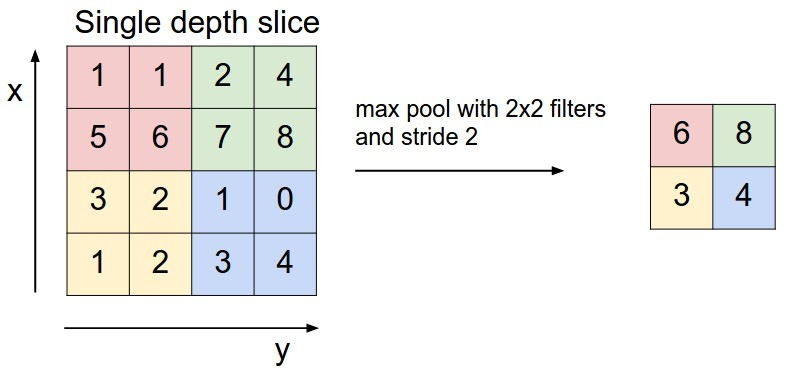
\includegraphics[width=0.8\textwidth]{\path/maxpool.jpeg} 
 \caption{Max pooling: in uscita l'immagine avrà 1/4 dei pixel di partenza.}
 \label{fig:maxpool}
\end{figure}
Attraversando la rete si avrà gradualmente un numero di feature maps  più alto e quindi della ricchezza della rappresentazione delle features; ed una diminuzione della risoluzione dell'input. Questi fattori combinati insieme donano un forte grado di invarianza alle trasformazioni geometriche dell'input.
 
\subsection{Strato completamente connesso (FC)}
%% menzionare che adesso si usa la convoluzione %% 
Nello strato completamente connesso, tutti gli input provenienti dai layer di convoluzione vengono dati in ingresso ad una normale rete neurale completamente connessa che fungerà da classificatore. I calcoli in questa parte finale sono quindi uguali alle moltiplicazioni tra matrici visti nel Capitolo \ref{Capitolo2}. \\
Ultimamente però, si è notato che, eccetto per la modalità di connessione, questi neuroni sono funzionalmente identici a quelli dei layer di convoluzione (entrambi computano moltiplicazioni fra matrici). Quindi si possono sostituire con degli strati di convoluzione che hanno un receptive field di 1x1\parencite{WCS231layer}. 

In figura \ref{fig:cnn4} è rappresentata l'architettura completa di una CNN. Si noti come la risoluzione dell'immagine si riduca ad ogni strato di pooling (chiamato anche subsampling) e come ogni pixel delle feature maps derivi dal campo recettivo sull'insieme di tutte le feature maps del livello precedente. \\
In figura \ref{fig:cnn3} invece, si può osservare una CNN nell'atto di classificazione di un'auto. Sono visualizzati i filtri della rete durante tutti i vari livelli di elaborazionde dell'input, per poi terminare in uno strato completamente connesso che da in output una probabilità. Questa probabilità è poi tradotta in uno score, da cui si sceglie la classe vincente. 
\begin{figure}[h!]
 \centering
 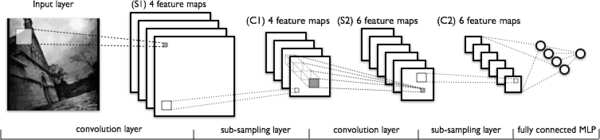
\includegraphics[width=1.0\textwidth]{\path/cnn-architecture.png} 
 \caption{Architettura di una CNN}
 \label{fig:cnn4}
\end{figure}

\begin{figure}[h!]
 \centering
 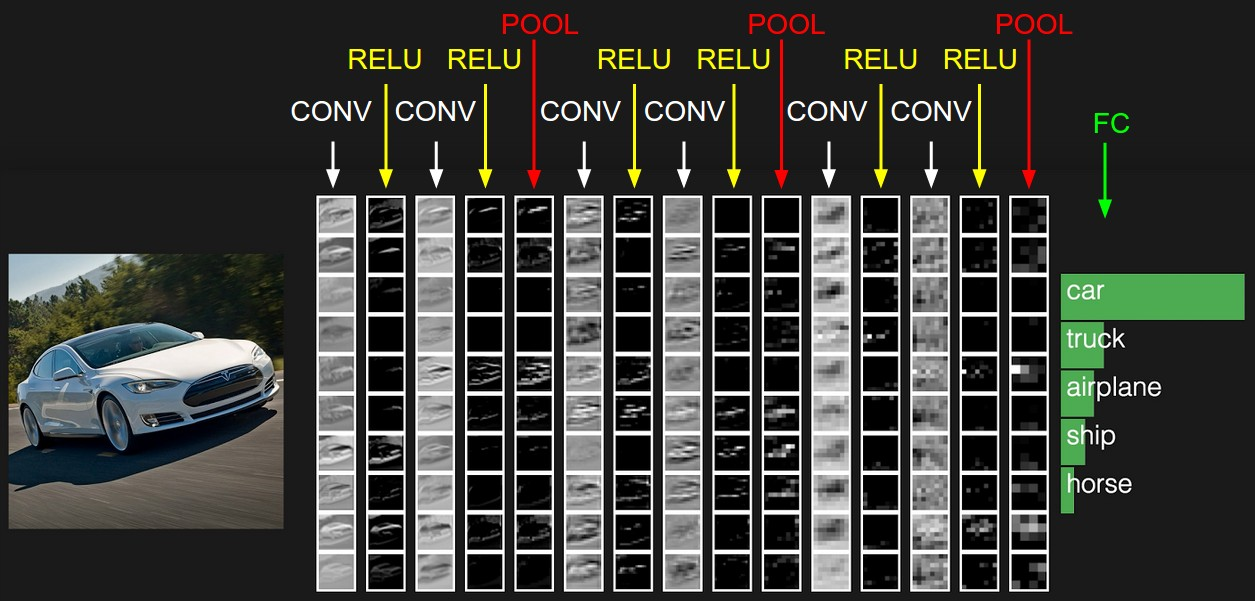
\includegraphics[width=1.0\textwidth]{\path/convnet.jpeg} 
 \caption{Tipica CNN in un task di classificazione; la classe vincente è quella con la probabilità più alta, indicata alla fine}
 \label{fig:cnn3}
\end{figure}
%--------------------------------------------------------------------
%	SECTION 3
%--------------------------------------------------------------------
\section{Applicazioni e risultati}
L'alta efficacia, la peculiare, vantaggiosa architettura insieme con l'enorme progresso tecnologico dell'hardware, hanno reso le CNN il sistema più promettente per compiti di visivo, con i più svariati ambiti applicativi come: riconoscimento e tagging facciale (si pensi a Facebook), ricerca intelligente di immagini (si pensi a Google Photos), automobili autonome, smartphone, robot, droni, (video)giochi ed altro. Le CNN hanno avuto eccellenti risultati anche nell'elaborazione naturale del linguaggio; nella scoperta di farmaci, poiché predicendo le interazioni tra determinate molecole e proteine hanno contribuito a scoprire potenziali biomolecole per il trattamento dell'ebola\parencite{WCNN}, tanto per citarne altri.\\
Già 3 anni fa, in un articolo pubblicato dal dipartimento di visione artificiale del KTH \parencite{Overfeat}, ha utilizzato ”OverFeat”, una CNN pubblica allenata per ILSVRC13, una competizione annuale di riconoscimento degli oggetti. L'articolo sottolinea come abbiano utilizzato questa CNN “off-the-shelf” ovvero già pronta e, senza allenarla ulteriormente, testandola contro altri metodi allo stato dell'arte finemente perfezionati sviluppati fino ad allora. Come test hanno scelto attività gradualmente sempre più lontane dall'originario compito per cui OverFeat è stata addestrata e, con enorme stupore, hanno verificato che OverFeat surclassa i suddetti metodi su qualsiasi dataset (si rimanda all'articolo per i dettagli) nonostante sia stata allenata solo mediante l'ImageNet. L'articolo si chiude con una frase che qui cito:
\begin{quote}
\emph{“Thus, it can be concluded that from now on, deep learning with CNN has to be considered as the primary candidate in essentially any visual recognition task.”}
\end{quote}\\
\subsection{Confronto con l'uomo}
Nel 2011, le CNN hanno la prima volta battuto l’uomo raggiungendo un errore di 0.56\% contro l’1.16\% degli umani sul riconoscimento dei segnali stradali nella competizione “German Traffic Sign competition run by IJCNN 2011”.\\
Un altro compito che è sempre stato difficile per la visione artificiale era il riconoscimento di visi parzialmente occlusi, capovolti o spostati di diverse angolazioni. Tuttavia, nel 2015 un team del Yahoo Labs, è riuscito a far apprendere anche questo compito ad una CNN\parencite{WMit}.

L'ultima pietra migliare in ordine cronologico della sfida "Uomo vs. Macchina" è senza dubbio quella di \textsc{AlphaGo}\parencite{WAlphaGo}. AlphaGo è il primo programma a riuscire a battere un giocatore umano professionista (Lee Sedol, 18 volte campione del mondo) all'antico gioco cinese di Go. \\
Go è conosciuto per essere computazionalmente estremamente complesso: vi sono $10^{170}$ possibili combinazioni della scacchiera, un numero più alto degli atomi dell'Universo conosciuto. È quindi inaffrontabile con un approccio a "forza bruta". 
\\
AlphaGo si basa su una combinazione di deep learning + tree search. In particolare, utilizza 3 CNN: 2 "policy network" per scegliere la strategia più vincente ed 1 "value network" come funzione euristica per valutare la bontà di un'ipotetica mossa. In più, l'output di queste reti è combinato con una "Montecarlo Tree Search" per avere una risposta finale sulla prossima mossa da giocare. Maggiori dettagli si trovano sul lungo paper pubblicato da DeepMind\parencite{AlphaGo}. \\
\\
Questi risultati bastano per comprendere la potenzialità delle convolutional neural networks.
